\part[Growing The Language]{Growing The Language}
\section{Scala's Hierarchy}
\begin{frame}{Scala's Hierarchy}
\begin{center}
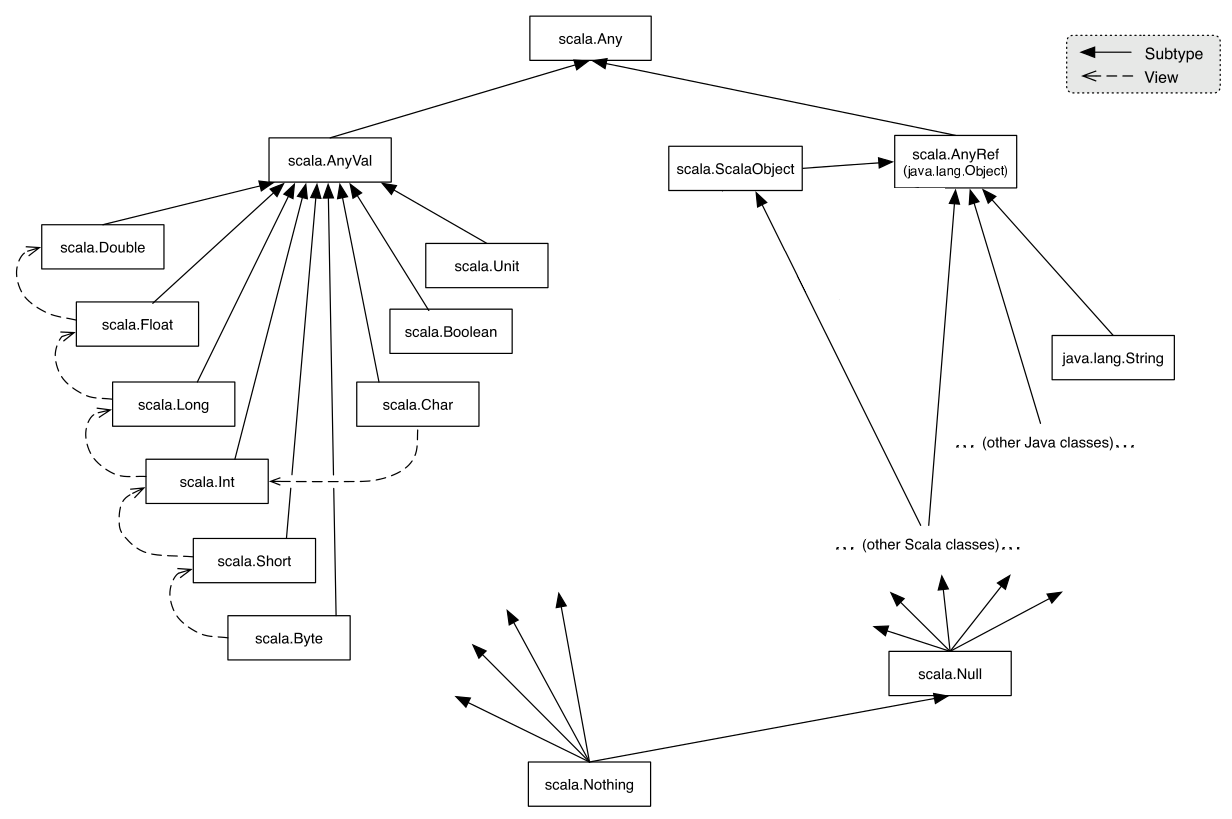
\includegraphics[width=\textwidth]{resources/Hierarchy.png}
\end{center}
\end{frame}

\begin{frame}[fragile]{``Any value'' is an object in Scala}
\begin{block}{\lstinline!Any!}
Because every class inherits from \lstinline!Any!, every object in a Scala
program can be compared using \lstinline!==!, !=, or
\lstinline!equals!; hashed using \lstinline!hashCode!; and formatted using
\lstinline!toString!. (\lstinline!==! always forwards to equals!)
\pause
\end{block}
\begin{lstlisting}
final def ==(that: Any): Boolean
final def !=(that: Any): Boolean
def equals(that: Any): Boolean
def hashCode(): Int
def toString(): String
def isInstanceOf[T]: Boolean
def asInstanceOf[T]: T
\end{lstlisting}
\pause
\begin{exampleblock}{Example}
\lstinline!1.toString == "1"!\\
\lstinline!"1".toInt  == 1.hashCode!
\end{exampleblock}
\end{frame}

\begin{frame}{Bottom types}
\begin{center}
Bottom types are just a workaround that handles some ``corner cases'' of Scala's
object-oriented type system in a uniform way
\end{center}
\end{frame}

\begin{frame}[fragile]{Null}
\begin{center}
Class \lstinline!Null! is the type of the \lstinline!null! reference; it is a
subclass of every reference class (i.e., every class that itself inherits from
\lstinline!AnyRef!). \lstinline!Null! is not compatible with \alert{value
types}. You cannot, for example, assign a \lstinline!null! value to an integer
variable:
\end{center}
\pause
\begin{alertblock}{\lstinline!Null! is for \lstinline!AnyRef!}
\begin{lstlisting}
scala> val i: Int = null
<console>:7: error: type mismatch;
 found   : Null(null)
 required: Int
\end{lstlisting}
\end{alertblock}
\end{frame}

\begin{frame}[fragile]{Null}
\begin{block}{Value types can be compared with null though}
\begin{lstlisting}
scala> 1 == null
<console>:8: warning: comparing values of types Int and Null
using == will always yield false
              1 == null
                ^
res0: Boolean = false

scala> null == 1
<console>:8: warning: comparing values of types Null and Int
using == will always yield false
              null == 1
                   ^
res1: Boolean = false
\end{lstlisting}
\end{block}
\end{frame}

\begin{frame}[fragile]{Null}
\begin{center}
Every method defined on \lstinline!Null! throws a
\lstinline!java.lang.NullPointerException! when invoked
\end{center}
\pause
\begin{exampleblock}{Exception for \lstinline!==!}
\begin{lstlisting}
scala> "abc" == null
res0: Boolean = false

scala> null == "abc"
res1: Boolean = false
\end{lstlisting}
\end{exampleblock}
\end{frame}

\begin{frame}{Nothing}
\begin{center}
Type \lstinline!Nothing! is at the very bottom of Scala�s class hierarchy; it is
a subtype of every other type. However, there exist \alert{no values} of this
type whatsoever
\end{center}
\end{frame}

\begin{frame}[fragile]{Nothing - Use case: signal abnormal termination}
\pause
\begin{lstlisting}
scala> val up = new Exception
up: java.lang.Exception = java.lang.Exception
\end{lstlisting}
\pause
\begin{lstlisting}
scala> def ralph = throw up
ralph: Nothing
\end{lstlisting}
\pause
\begin{lstlisting}
scala> def whatsItGonnaBe(sober: Boolean) =
     |    if(sober) "keep drinking" else ralph
whatsItGonnaBe: java.lang.String
\end{lstlisting}
\pause
\begin{lstlisting}
scala> println(whatsItGonnaBe(sober = true))
keep drinking

scala> println(whatsItGonnaBe(sober = false))
java.lang.Exception
        at .<init>(<console>:7)
        ...
\end{lstlisting}
\end{frame}

\begin{frame}[fragile]{Nothing}
\begin{exampleblock}{\lstinline!Nothing! in Java}
\begin{lstlisting}[language=Java]
int divide(int x, int y) {
   if (y != 0) return x / y;
   else throw new RuntimeException();
}
\end{lstlisting}
\end{exampleblock}
\pause
\begin{alertblock}{\lstinline!Nothing! in Java}
\begin{lstlisting}[language=Java]
int divide(int x, int y) {
   return y != 0 ? x / y : throw new RuntimeException();
}
\end{lstlisting}
Multiple markers at this line:
\begin{itemize}
  \item Syntax error on token ``throw'', delete this token
  \item Type mismatch: cannot convert from Serializable to int
\end{itemize}
\end{alertblock}
\end{frame}

\section{Growing Types}
\begin{frame}[fragile]{Operators}
\begin{block}{What is an operator?}
\pause
Operator is a convenient \highlight{notation} for an operation call
\end{block}
\pause
\begin{exampleblock}{Unary operators}
\begin{description}
\item[prefix] \lstinline!-4711!
\item[postfix] \lstinline!1337 toString // avoid postfix notation!
\end{description}
\end{exampleblock}
\pause
\begin{exampleblock}{Binary (infix) operators}
\begin{lstlisting}
1 == 1 // true
1 equals 1 // true
1 != 1 // false
\end{lstlisting}
\end{exampleblock}
\pause
\begin{center}
\highlight{Every method in Scala can be invoked using the operator notation}
\end{center}
\end{frame}

\begin{frame}[fragile]{Operators}
\begin{exampleblock}{Every method is an operator}
\begin{lstlisting}
scala> 1 + 2
res0: Int = 3

scala> (1).+(2)
res1: Int = 3
\end{lstlisting}
\end{exampleblock}
\pause
\center{Parenthesis can be omitted in most cases, but\ldots}
\begin{alertblock}{Be aware of dots}
\begin{lstlisting}
scala> 1.+(2)
res0: Double = 3.0

scala> 1. + 2
res1: Double = 3.0
\end{lstlisting}
\end{alertblock}
\end{frame}

\begin{frame}[fragile]{Operators}
\begin{alertblock}{Be aware of lambdas}
\begin{lstlisting}
scala> List(1,2,3) map x => x * x
<console>:1: error: not a legal formal parameter
       List(1,2,3) map x => x * x
                   ^
\end{lstlisting}
\end{alertblock}

\begin{exampleblock}{Be aware of lambdas}
\begin{lstlisting}
scala> List(1,2,3) map (x => x * x)
res0: List[Int] = List(1, 4, 9)
\end{lstlisting}
\end{exampleblock}
\end{frame}

\begin{frame}[fragile]{Operators}
\begin{alertblock}{Be aware of the arity}
\begin{lstlisting}
scala> "Hello, world!" indexOf 'o', 5
<console>:1: error: ';' expected but ',' found
       "Hello, world!" indexOf 'o', 5
                                  ^
\end{lstlisting}
\end{alertblock}
\begin{exampleblock}{Be aware of the arity}
\begin{lstlisting}
scala> "Hello, world!" indexOf ('o', 5)
res0: Int = 8
\end{lstlisting}
\end{exampleblock}
\end{frame}

\begin{frame}[fragile]{Operators}
\begin{block}{Equality operators}
\begin{description}
\item[==] object equality
\item[equals] object equality
\item[!=] object inequality
\item[eq] reference equality (defined only for \lstinline!AnyRef!)
\item[ne] reference inequality (defined only for \lstinline!AnyRef!)
\end{description}
\end{block}
\pause
\begin{alertblock}{Exception for \lstinline!eq! with string literals}
\begin{lstlisting}
scala> "abc" eq "abc"
res0: Boolean = true
\end{lstlisting}
\end{alertblock}
\end{frame}

\begin{frame}[fragile]{Operators}
Methods are operators, therefore operators are methods. Methods can be
\highlight{lifted} to functions. This sometimes leads to \alert{scary} code like
this:
\begin{block}{Read it if you can}
\begin{lstlisting}
scala> val names = List("Martin", "John", "Martin")
names: List[java.lang.String] = List(Martin, John, Martin)

scala> names filter ( "Martin" == ) size
res0: Int = 2
\end{lstlisting}
\end{block}
\pause
\begin{exampleblock}{Easier to read}
\begin{lstlisting}
names filter ( "Martin" == _ )
names filter ( _ == "Martin" )
\end{lstlisting}
\end{exampleblock}
\end{frame}

\begin{frame}[fragile]{Operators}
\begin{block}{Identifiers have very few limitations\ldots}
\begin{description}
\item[prefix] only \lstinline!+!, \lstinline!-!, \lstinline!~! and \lstinline{!}
are allowed
\item[infix] almost any symbol is allowed
\item[postfix] almost any symbol is allowed
\end{description}
\end{block}
\end{frame}

\begin{frame}[fragile]{Operators}
\begin{block}{Prefix operators have to be prefixed with \lstinline!unary_!}
\begin{lstlisting}
scala> class Number(val x: Int) {
     |    def unary_- : Number = new Number(-x)
     |    override def toString = x.toString
     | }
defined class Number

scala> val ten = new Number(10)
ten: Number = 10

scala> val minusTen = -ten
minusTen: Number = -10
\end{lstlisting}
\end{block}
\end{frame}

\begin{frame}{Operators - Precedence}
\begin{center}
Operator precedence determines which parts of an expression are evaluated before
the other parts. Scala decides precedence based on the first character of the
methods used in operator notation
\end{center}
\begin{block}{Operator precedence}
\begin{center}
\begin{tabular}{l}
(all other special characters)\\
* / \%\\
+ -\\
:\\
= !\\
$< >$\\
\&\\
$\wedge$\\
$|$\\
(all letters)\\
(all assignment operators)\\
\end{tabular}
\end{center}
\end{block}
\end{frame}

\begin{frame}[fragile]{Operators - Precedence}
\begin{alertblock}{Exception - assignment operators}
If an operator ends in an equals character (\lstinline!=!), and the operator is
not one of the comparison operators \lstinline!<=!, \lstinline!>=!,
\lstinline!==!, or \lstinline!=!, then the precedence of the operator is the
same as that of simple assignment (\lstinline!=!). That is, it is lower than the
precedence of any other operator.
\end{alertblock}
\begin{exampleblock}{Exception - assignment operators}
\begin{lstlisting}
x *= y + 1
// means the same as:
x *= (y + 1)
\end{lstlisting}
\end{exampleblock}
\end{frame}

\begin{frame}[fragile]{Operators - Associativity}
When multiple operators of the same precedence appear side by side in
an expression, the \highlight{associativity} of the operators determines the way
operators are grouped. The associativity of an operator in Scala is determined by its
\highlight{last} character:
\begin{block}{Associativity}
\begin{description}
  \item[right-associative] any method that ends in a '\lstinline!:!'
  \item[left-associative] any method that ends in any other character, than
  '\lstinline!:!'
\end{description}
\end{block}
\begin{exampleblock}{Associativity}
\begin{lstlisting}
a * b // is invoked as a.*(b)
a : b // is invoked as b.:(a)
\end{lstlisting}
\end{exampleblock}
\end{frame}

\begin{frame}[fragile]{Operators - Associativity}
\begin{exampleblock}{Few right-associative examples from the Scala collections
library}
\begin{lstlisting}
scala> 1 :: 2 :: Nil == List(1, 2)
res0: Boolean = true
\end{lstlisting}
\pause
\begin{lstlisting}
scala> 1 :: 2 :: Nil ::: List(3, 4) == List(1, 2, 3, 4)
res1: Boolean = true
\end{lstlisting}
\pause
\begin{lstlisting}
scala> (0 /: List(1, 2, 3))( _ + _ )
res2: Int = 6

// is the same as

scala> List(1, 2, 3).foldLeft(0)( _ + _ )
res3: Int = 6
\end{lstlisting}
\end{exampleblock}
\end{frame}

\begin{frame}{Scala - the pure OO language}
\begin{center}
Scala is an object-oriented language in pure form: every \highlight{value} is an
\highlight{object} and every \highlight{operation} is a \highlight{method call}
\end{center}
\end{frame}

\section{Growing Control Structures}
\begin{frame}{Growing Control Structures}
\begin{block}{Why do we need control abstractions?}
\pause
\begin{enumerate}
  \item to reduce code duplication
  \item to make client code more concise
\end{enumerate}
\end{block}
\end{frame}

\begin{frame}{Strategy pattern}
\begin{block}{What is the strategy pattern?}
\pause
The strategy pattern defines a family of algorithms, encapsulates each one, and
makes them interchangeable. Strategy lets the algorithm vary independently from
clients that use it.
\end{block}
\pause
\begin{block}{Higher-order functions revisited}
All functions are separated into common parts, which are the same in every
invocation of the function, and non-common parts, which may vary from
one function invocation to the next. The common parts are in the body of
the function, while the non-common parts must be supplied via arguments.
When you use a function value as an argument, the non-common part of
the algorithm is itself some other algorithm!
\end{block}
\end{frame}

\begin{frame}[fragile]{Strategy pattern in action}
\onslide<1->\begin{lstlisting}
def containsNeg(nums: List[Int]): Boolean = {
   var exists = false
      for (num <- nums)
\end{lstlisting}
\onslide<1->\lstinline!          if (!\onslide<2->\lstinline!num < 0!\onslide<1->\lstinline!)!
\onslide<1->\begin{lstlisting}
            exists = true
      exists
}

def containsOdd(nums: List[Int]): Boolean = {
   var exists = false
      for (num <- nums)
\end{lstlisting}
\onslide<1->\lstinline!          if (!\onslide<2->\lstinline!num % 2 == 1!\onslide<1->\lstinline!)!
\onslide<1->\begin{lstlisting}         
            exists = true
   exists
}
\end{lstlisting}
\end{frame}

\begin{frame}[fragile]{Strategy pattern in action}
\begin{lstlisting}
def containsNeg(nums: List[Int]) = nums exists (_ < 0)

def containsOdd(nums: List[Int]) = nums exists (_ % 2 == 1)
\end{lstlisting}
\end{frame}

\begin{frame}[fragile]{Loan pattern}
\begin{block}{What is the loan pattern?}
\pause
The loan pattern ensures that a resource is deterministically disposed of
(closed) once it goes out of scope
\end{block}
\pause
\begin{exampleblock}{Loan pattern in Java}
\begin{lstlisting}[language=java]
SomeResource resource = new SomeResource();
try {
   resource.doSomethingUseful();
}
finally {
   if (resource != null)
      resource.close();
}
\end{lstlisting}
\end{exampleblock}
\end{frame}

\begin{frame}[fragile]{Loan pattern}
\begin{exampleblock}{Loan pattern in C\#}
\begin{lstlisting}[language=cSharp]
using (var resource = new SomeResource())
{
   resource.DoSomethingUseful();
}
\end{lstlisting}
\end{exampleblock}
\pause
\begin{exampleblock}{Loan pattern in Scala (as soon as we finish implementing
it)}
\begin{lstlisting}
using (new SomeResource) {
   _.doSomethingUseful()
}
\end{lstlisting}
\end{exampleblock}
\end{frame}

\begin{frame}[fragile]{Implementing the loan pattern - Part 1}
\begin{exampleblock}{Implementation}
\onslide<1->\lstinline!object LoanPattern {!\\
\onslide<2->\lstinline!   def using!\onslide<4->\lstinline![R <: { def close() }]!\\
\onslide<3->\lstinline!      (resource: R, operateOn: R => Unit)!\onslide<2->\lstinline!: Unit = {!\\
\onslide<5->\lstinline!          try operateOn(resource)!\\
\onslide<6->\lstinline{          finally if (resource != null) resource.close()}\\
\onslide<2->\lstinline!   }!\\
\onslide<1->\lstinline!}!\\
\end{exampleblock}
\onslide<7->
\begin{exampleblock}{Call}
\lstinline!import LoanPattern.using!
\lstinline!using (new SomeResource, _.doSomethingUseful())!
\end{exampleblock}
\end{frame}

\begin{frame}[fragile]{Implementing the loan pattern - Part 2}
\begin{exampleblock}{Implementation}
\onslide<1->\begin{lstlisting}
object LoanPattern {
   def using[R <: { def close() }]
      (resource: R)(operateOn: R => Unit): Unit = {
         try operateOn(resource)
         finally if (resource != null) resource.close()
   }
}
\end{lstlisting}
\end{exampleblock}
\onslide<2->
\begin{exampleblock}{Call}
\lstinline!import LoanPattern.using!
\lstinline!using (new SomeResource)(_.doSomethingUseful())!
\onslide<3->\lstinline!using (new SomeResource){_.doSomethingUseful()}!
\onslide<4->\lstinline!using (new SomeResource) {!\\
\onslide<4->\lstinline!   _.doSomethingUseful()!\\
\onslide<4->\lstinline!}!
\end{exampleblock}
\end{frame}

\begin{frame}[fragile]{By-name parameters}
\begin{center}
We would like to implement a control abstraction, which we will call
\lstinline!loop!. It will have \highlight{two} parameter lists. Each of them
takes only \highlight{one} argument. The first parameter list will take a
function of type \lstinline!() => Unit!. The second parameter list will take a
number of type \lstinline!Int!. The control abstraction should simply invoke the
\highlight{function} a \highlight{number} of times\ldots
\end{center}
\end{frame}

\begin{frame}[fragile]{Implementing \lstinline!loop! - Part 1}
\begin{exampleblock}{Implementation}
\begin{lstlisting}
def loop(function: () => Unit)(number: Int): Unit = {
   for (i <- 1 to number)
      function()
}
\end{lstlisting}
\end{exampleblock}
\pause
\begin{exampleblock}{Call}
\begin{lstlisting}
loop {
   () => println("Hello, World!")
}(10)
\end{lstlisting}
\end{exampleblock}
\end{frame}

\begin{frame}[fragile]{Implementing \lstinline!loop! - Part 2}
\begin{exampleblock}{Implementation}
\begin{lstlisting}
def loop(function: => Unit)(number: Int): Unit = {
   for (i <- 1 to number)
      function
}
\end{lstlisting}
\end{exampleblock}
\begin{exampleblock}{Call}
\begin{lstlisting}
loop {
   println("Hello, World!")
}(10)
\end{lstlisting}
\end{exampleblock}
\end{frame}

\section{Summary}
\begin{frame}{Summary}
\begin{itemize}
  \item Scala is very \highlight{consistent}
  \item ``Everything'' is an \highlight{expression}
  \item ``Every'' expression yields a \highlight{value} and all values have
  \highlight{types}
  \item ``Every'' value is an \highlight{object}
  \item ``Every'' operation is a \highlight{method call}
  \item Operator is just a \highlight{notation} for an operation call
  \item ``Everything'' can be compared with \lstinline!==!
  \item Features like native support for \highlight{higher-order functions},
  \highlight{function currying} or \highlight{by-name parameters} make your own
  abstractions feel as built-in control structures and thus let you grow the
  language to your needs\ldots
\end{itemize}
\end{frame}